\chapter{Forschungsstand}
\label{sec:S3_Forschungsstand}

\section{Gamification}
\label{subsec:S3_Gamification}

Der Begriff Gamification geht auf Nick Pelling 2002 zurück.
Er beschreibt den Prozess bei dem Spielmechaniken auf bestehende Aspekte angewendet werden um eine extrinsische Motivation zu erzeugen.\citep{Marczewski.2013}
Erste Gamification Ansätze gab es bereits zu Beginn des 20. Jahrhunderts z.B. durch Stempelkarten an der Eisdiele. Später wurden ähnliche Konzepte in Vielfliegerprogrammen aufgegriffen.
In der Literatur gibt es unterschiedliche Definitionen der Gamification.
In der nachfolgenden Tabelle \ref{img:ch3_table_definitions.png}

\begin{table}
\tiny
    \begin{tabular}{llllll}
    ~                         & Zichermann,Cunningham (2011) & Detering et al. (2011) & Breuer (2011) & Oxford (2013) & Kapp (2012) \\
    Nutzung von Spielmechanik & X                             & X                      & X             & X             & X           \\
    Motivation                & X                             & ~                      & ~             & ~             & X           \\
    Problemlösung             & X                             & ~                      & ~             & ~             & X           \\
    Spielferner Kontext       & ~                             & X                      & X             & X             & ~           \\
    Verhaltensbeinflussung    & ~                             & ~                      & X             & ~             & ~           \\
    Lernförderung             & ~                             & ~                      & ~             & ~             & X           \\
    Anregung zum Handeln      & ~                             & ~                      & ~             & ~             & X           \\
    \end{tabular}
    \caption{Literaturübersicht zur Definition von Gamification}
\end{table}

Es gibt verschiedene Definitionen:

-Definition von Gamification:

Oxford:
"the application of typical elements of game playing (e.g. point scoring, competition with others, rules of play) to other areas of activity, typically as an online marketing technique to encourage engagement with a product or service:
gamification is exciting because it promises to make the hard stuff in life fun"

"The process of game-thinking and game mechanics to engage users and solve problems"
(Zichermann, Cunningham (2011, S. XIV)

"Gamification is the use of game design elements in non-game context"
(Deterding, Dixon et al. (2011, S2.)

Kapp "Gamification is using game based mechanics, aesthetics and game thinking to engange people, motivate action, promote learning, and solve problems"
Kapp, 2012, S.10


"From Game Design Elements to Gamefulness: Defining Gamification" - (SEBASTIAN, DAN, RILLA and LENNART 2011):


ODOBSAIC et. al Gamificatoin of geographic data collection (2013):

\begin{figure}[H]
\begin{center}
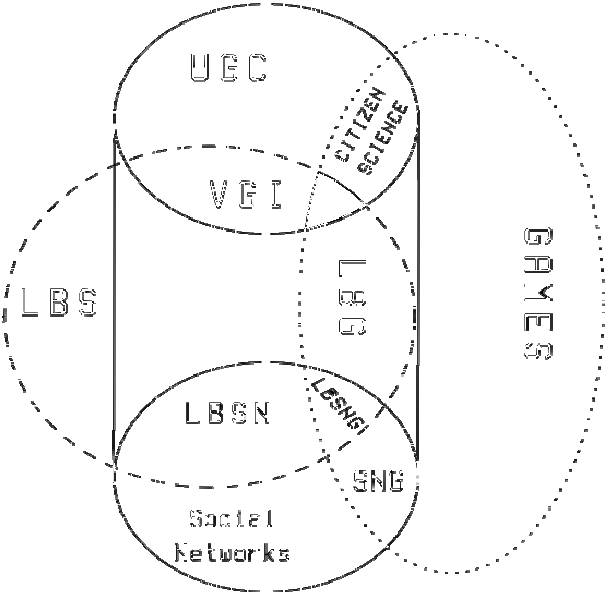
\includegraphics[width=80mm]{images/ch3_img01_LBG_SN_etc.png}
\caption{Einordnung Definition}
\label{img:ch3_img01_LBG_SN_etc}
\end{center}
\end{figure}

\begin{figure}[H]
\begin{center}
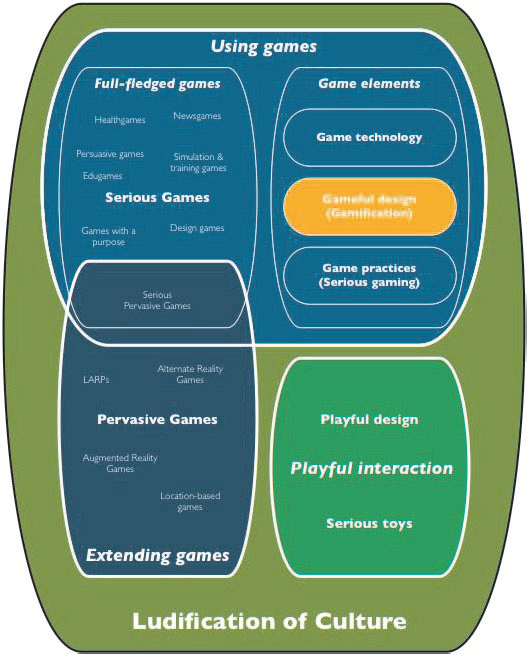
\includegraphics[width=80mm]{images/ch3_img02_gamification.png}
\caption{Gamification @ Deterding et. al}
\label{img:ch3_img01_LBG_SN_etc}
\end{center}
\end{figure}

Bei allen:
Nutzung von Spieldenken und Spielmechaniken

Bei Zichermann \& Kapp:
Motivatoin \& Problemlösung

aber auch "Empowerement":
Games have a strong ability of imparting a sense of agency to the players, making them feel
empowered and giving them the impression that their decisions are meaningful and will
have an impact. A sense of agency refers to the subjective awareness that one is initiating,
executing and controlling one’s own volitional actions in the world (JEANNEROD 2003).

Sonst:
Spielferner Context
Lernförderung, Anregung zum Handeln

-Es werden verschiedne Elemente genutzt um Spieler zu spielfremden Verhalten (hier: Besuch von Geschäften) zu motivieren


Zichermann \& Cunningham (2011):
Mensch hat Hang zum Spielen.

SAPS (do not give something for free, but something for status etc.)

\begin{itemize}
      \item Status (Badges, Levels, Leaderboards)
      \item Access (early Access)
      \item Power (give power, e.g. modicum control over other players)
      \item Stuff (give a reward, try to prevent that the price gets known)
\end{itemize}

The house always wins

"flow"
Game designers aim to
keep a player in a constant state of flow. Flow indicates the state in which a player is between
anxiety and boredom and meeting their own motivational level in that experience
(Csíkszentmihályi 1991).

Game Mechanics:
\begin{itemize}
      \item Points
      \item Levels
      \item Leaderboard
      \item Badges
      \item Challenges
      \item Onboarding
      \item engagement loops
\end{itemize}

Der Begriff Gamification wird aktiv seit ca. 2010 genutzt. Die Ansätze sind bereits seit den 80ern in Verwendung und per se nichts neues.
Es gibt unterschiedliche Definitionen für diese Arbeit wird ein Fokus auf die Terminologie von Zichermann gelegt, da dieser darüber hinaus ein strukturiertes Modell für einzelene Elemente der Gamification bietet.

\section{Geogames}
\label{subsec:S3_Geogames}

Game/Spiel:

According to  Katie  Salen  and  Eric  Zimmerman  (2004): "Magic circle"

Mobilegames
-games played on mobile devices (Bell et al. 2006)

Locationbased Games
games played in a location context
Kiefer et al. 2006, Benford et al. 2003
"Extending Cyberspace: Location Based Games Using Cellular Phones":
Rashid 2006

Geogames:
Schlieder et al. 2006

Pervasive Games

bluring the magic circle in "Montola, Markus. "Exploring the edge of the magic circle: Defining pervasive games." Proceedings of DAC. 2005."

"A pervasive game is agame that has one or more salient features that expand the 
contractual magie circle of play spatially, temporally, or socially. " @ Motola et al 2009

" This   definition   has   been   discussed   earlier  in   Montola   (2005)   and   in   Montola,   Waern,   and 
Nieuwdorp  (2006).  Staffan  Björk  (2007)  has  also  published  an  alternate version,  where  ambiguity 
of  interaction or  interface is  included  as  a  fourth  central  defining ceriterion." 

Can You See Me Now (CYSMN) (Flintham et al., 2003a)
GeoTicTacToe and CityPoker (see Schlieder et al. 2005a, Schlieder 2005b)
Human Pacman, realised by Choek et al. (2004)

Unterscheidung zwischen LBG, AR MR etc:

Concepts and Technologies for Pervasive Games (A reader for pervasive gaming research) (Hinske et al., 2007)

Es gibt viele verschiedene umgesetzte Spiele im Geogames/Pervasive Gaming Bereich

\section{Relokalisierungsansätze}

Generell was ist eine Location?
Wodurch wird diese definiert?


Literatur von KInf, sonst keine in diesem Umfeld.
Relocalisierungsansätze werden zwar angesprochen, z.B. in 
Exploring the Edge of the Magic Circle: 
Defining Pervasive Games 
Markus Montola 

es wird auf eventuelle Implikationen hingewiesen aber nicht im Detail weiter verfolgt.

Mannara 2012 ist ein erster Ansatz für ein Framework zu Relokalisierung von Spielfeldern basierend auf OSM Daten aber mit Fokus auf Eclipse EMF

\section{Verwendung offener Geodaten}
\label{subsec:S3_offeneGeodaten}

Hier: Was ist unter offen zu verstehen?

Es gibt zwei Bezugsquellen von öffentlichen Daten.
Zunächst die Daten welche von bestimmten Städten (vgl. Wien, Berlin, München) oder Ländern (Dänemark) den Bürgern zur Verfügung gestellt werden. Die Art, Qualität, sowie Umfang der Daten unterscheiden sich jedoch erheblich.

Eine zweite Option sind von offene (Geo-)Datenbanken, welche von privaten Personen durch Mapping oder externe lizenzierte Quellen zusammen gesammelt wurden. Eine dieser Datenbanken ist OpenStreetMap (OSM).


Haklay, Mordechai. "How good is volunteered geographical information? A comparative study of OpenStreetMap and Ordnance Survey datasets." Environment and planning. B, Planning \& design 37.4 (2010): 682.

\&

"Quality Assessment of the French OpenStreetMap Dataset" Girres et al. (2010)

Ergebnis:

Qualität der Daten von OSM hat seit dem Start (2004) enorm zugenommen, je nach Land besteht eine höhere Abdeckungsrate. Zur Zeit gibt es ca 20.000 aktive Mapper.

Mapping in Städten deutlich genauer wie "auf dem Land/außerhalb".  avg. distance ~1 vs ~30m.

Es gibt eine generelle Ungenauigkeit bei den Namen der Objekte.

Logische Konsistenz im Modell von OSM nicht verhanden.

Hecht 2013:
-Abdeckung/Coverage relativ gering, allerdings Genauigkeit proportional zu Stadtgröße

Pfoser et al. 2013:
-zwar teilweise gernige coverage, aber sehr hohe Klassifikationsrate, bei dennoch hoher Fehlerate von bis zu 23%
